\section{Alte menționări}
\subsection{Unde poate fi găsit acest atestat?}\label{links}
Am publicat acest atestat, pentru a face lucrurile mai ușoare pentru mine atunci când am lucrat la el, dar și pentru a putea să îl distribui pe internet, dacă cineva dorește să îl folosească, pe GitLab, dar și pe GitHub:

\begin{center}
 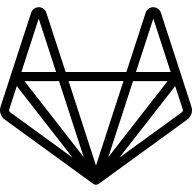
\includegraphics[height=\fontcharht\font`\B]{logos/gitlab}
 \url{gitlab.com/Andy3153/atestat_informatica}
  
 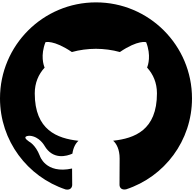
\includegraphics[height=\fontcharht\font`\B]{logos/github}
 \url{github.com/Andy3153/atestat_informatica}
\end{center}

\subsection{Fontul folosit în program}
Pentru întreaga interfață a calculatorului (textul butoanelor/textul display-ului), am folosit fontul Iosevka (patch-uit cu Nerd Fonts) (\url{github.com/ryanoasis/nerd-fonts/tree/master/patched-fonts/Iosevka}). Va trebui instalat și acesta pentru ca programul să compileze.

\subsection{Pentru compilarea documentației cu \LaTeX}
Pentru a compila documentația, pe lângă o distribuție de \LaTeX, cum ar fi \TeX\ Live, este nevoie să instalați și Pygments (\url{pygments.org}). Acesta este un program extern utilizat de pachetul \texttt{minted}, care este responsabil pentru afișarea codului în pagină.

De asemenea, este necesară folosirea opțiunii \texttt{-shell-escape} când este apelat programul \XeLaTeX\ (ex.: \texttt{xelatex -shell-escape file.tex})
